\documentclass[a4paper]{article}
\usepackage[margin=2cm]{geometry}
\usepackage[english]{babel}
\usepackage{graphicx, hyperref, longtable, amsmath, amssymb, csquotes, float, csvsimple, forloop}
\graphicspath{{../report/media/}{../result/}}

%% variables used in model
\newcommand{\ePR}{e_{PR}}
\newcommand{\eP}{e_P}
\newcommand{\gP}{g_P}
\newcommand{\aP}{a_P}
\newcommand{\eBR}{e_{BR}}
\newcommand{\eB}{e_B}
\newcommand{\gB}{g_B}
\newcommand{\mB}{m_B}

\begin{document}

\section{Scan details}
A new scan (11K simulations, $<$ 15 sec tuntime on laptop, 1 cpu) was performed with following parameter selection criteria:
\begin{itemize}
    \item biological parameters were categorized into two main groups: the fraction ($\ePR$, $\eP$, $\eBR$, $\eB$) and rate ($\gP$, $\mB$ \& $\aP$, $\gB$) groups
    \item ranges were calculated for parameters with $>$5 data points (i.e. $\ePR$, $\eP$, $\gP$, $\gB$) with $\gB$ having a parameter treatment
    \begin{itemize}
        \item $\gB$ in data is a growth rate ($day^{-1}$) but in model is a clearance rate ($\dfrac{m^3}{gC\cdot day}$)
        \item in data: clearance rate $\times$ resource density = growth rate
        \item as ``resource density" in this model is a variable while no such information in BioTrait data, it is given an arbitrary number (10 in this run) to result a seemingly ``normal-looking" growth rate $\gB$ in model
    \end{itemize}
    \item there is no single species data covered all the four (either phytoplankton or bacteria) biological parameters; hence the only meaningful approach is a very general coverage on every species
    \item number of data points collected from paper
    \begin{itemize}
        \item $\ePR$: 56*6 (it is calculated from $\gP$ by using the 6 temperature-standardised statistical models extracted; none of the species are in common)
        \item $\eP$: 13
        \item $\gP$: 56
        \item $\aP$: 3
        \item $\eBR$: 1
        \item $\eB$: 1
        \item $\gB$: 2333
        \item $\mB$: 1
    \end{itemize}
    \item percentage ranges of parameters with more than 5 data points were calculated and the largest range within each category (ranges of $\ePR$ and $\gP$ respectively)
    \item all parameter were ranged either according to the percentage ranges or their own (if available) or the ``umbrella range" of its category based on the mean of its available data value
    \item all simulated parameters values were selected from an uniform prior (as data is deficient in all parameters AND the use of Latin Hypercube Sampling technique)
    \begin{itemize}
        \item $x$: 0, 1 (wild scan) [$day^{-1}$]
        \item $\ePR$: 0.08, 0.87 (2 d.p.) [no unit]
        \item $\eP$: 0.4, 1 [no unit]
        \item $\gP$: 0.03, 3.17 (2 d.p.) [$day^{-1}$]
        \item $\aP$: 0.02, 1.52 (2 d.p.) [$\dfrac{m^3}{gC\cdot day}$]
        \item $\eBR$: 0.13, 1 (2 d.p.) [no unit]
        \item $\eB$: 0.07, 0.82 (2 d.p.) [no unit]
        \item $\gB$: 0.10, 3.50 (2 d.p.) [$\dfrac{m^3}{gC\cdot day}$]
        \item $\mB$: 0.01, 0.63 (2 d.p.) [$day^{-1}$]
    \end{itemize}
    \item the model was scripted in ``modIRL.R" file
\end{itemize}
Result was analysed in natural log; Wilcoxon rank sum tests were performed on each comparable pair of ``P-only" and ``P+B" systems

\section{System carbon distribution}
yield = organic carbon pool $\times$ removal rate (i.e. [$x$])\\
\newcounter{i0}
\forloop{i0}{1}{\value{i0}<10}{\includegraphics[width=\linewidth]{../result/sys_0\arabic{i0}.png}\\}
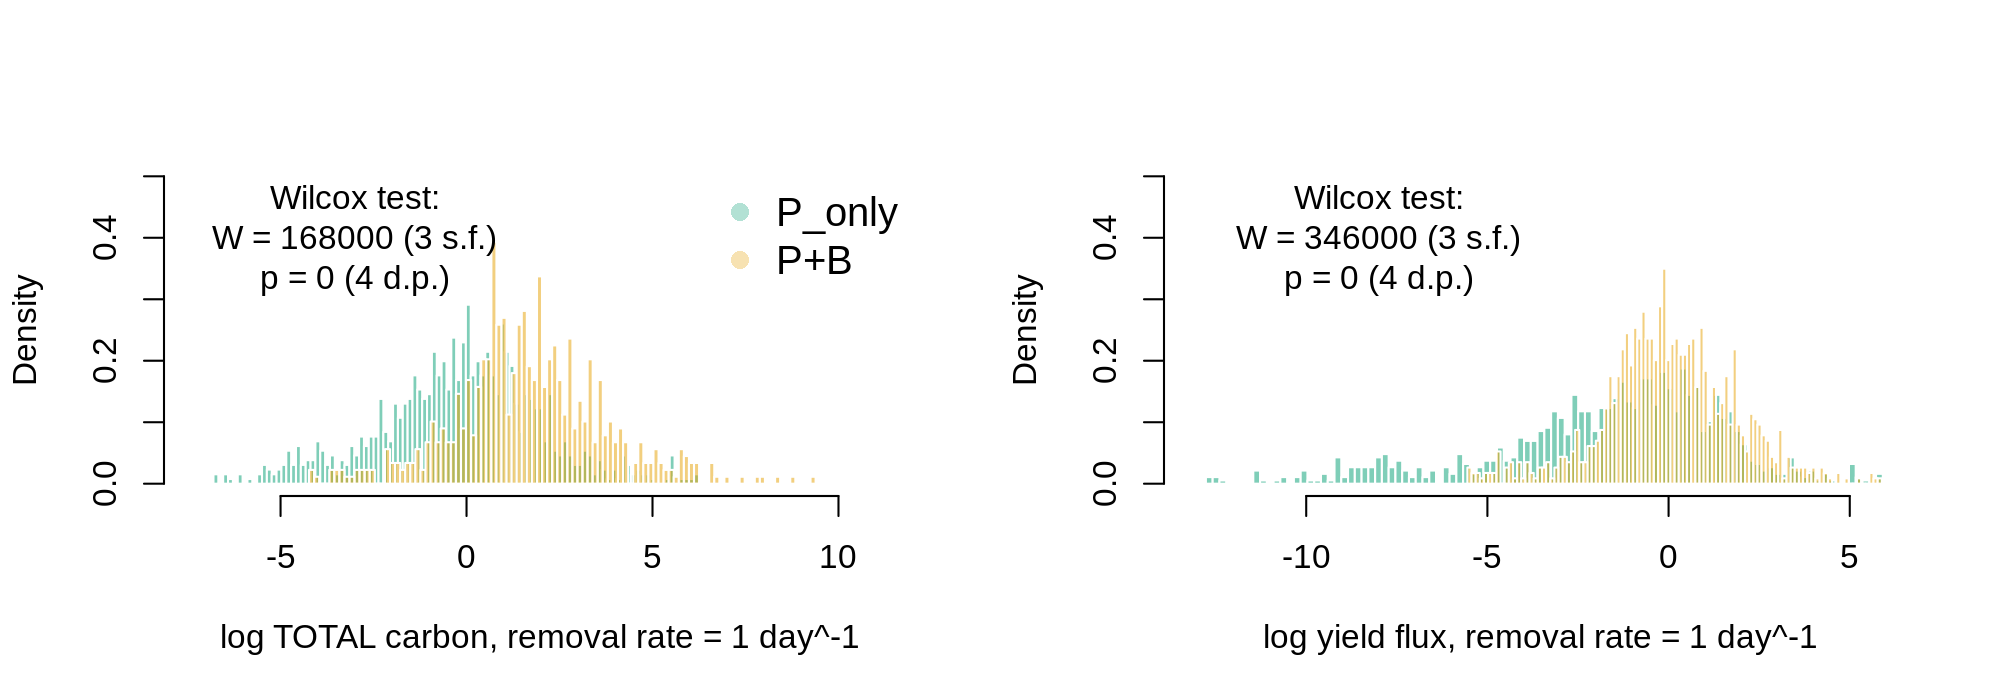
\includegraphics[width=\linewidth]{../result/sys_10.png}

\end{document}
